\mychapter{Metodologia}
\label{Cap:Metodologia}

Este capítulo aborda a metodologia aplicada no desenvolvimento do \textit{software}, quais métodos de engenharia de \textit{software} foram aplicados durante o processo, desde a concepção, até a prototipação

% -------------------------
\section{Metodologia de desenvolvimento do \textit{software} RADARE}

O desenvolvimento do \textit{software} RADARE adotou o método ágil Scrum como estrutura principal para orientar o processo de criação e entrega do produto \cite{softwareengreq}. Ele sendo uma metodologia ágil amplamente reconhecida, escolhido devido à sua capacidade de promover uma abordagem iterativa e flexível, especialmente adequada para uma equipe com um único desenvolvedor, como é o caso do desenvolvimento do RADARE \cite{scrum}.

Ao utilizar o Scrum, o desenvolvedor pôde organizar o trabalho em ciclos curtos e mensuráveis, conhecidos como "\textit{sprint}". Cada \textit{sprint}, com duração definida, permite ao desenvolvedor focar em metas claras e alcançáveis, priorizadas com base nas necessidades do projeto. Essa abordagem iterativa possibilitou uma resposta rápida a mudanças nos requisitos e uma entrega contínua de funcionalidades ao longo do desenvolvimento.
        
Para o desenvolvimento do \textit{software} RADARE, o Scrum facilita a gestão eficiente do projeto, com reuniões diárias para monitorar o progresso, identificar possíveis obstáculos e ajustar o plano conforme necessário. Além disso, as reuniões de revisão de \textit{sprint} permitem uma demonstração transparente das funcionalidades desenvolvidas, garantindo uma comunicação eficaz com \textit{stakeholders} e a validação contínua do produto.
        
A aplicação do método Scrum no desenvolvimento do \textit{software} RADARE não apenas proporciona uma estrutura organizacional clara, mas também promove uma cultura de colaboração e melhoria contínua. Ao enfatizar a transparência, a comunicação e o \textit{feedback}, o Scrum permite ao desenvolvedor adaptar-se rapidamente às mudanças no ambiente de desenvolvimento e priorizar o valor entregue ao cliente.
        
Em resumo, a escolha do método Scrum para o desenvolvimento do \textit{software} RADARE demonstrou ser uma decisão acertada. Sua flexibilidade, foco na entrega de valor e capacidade de adaptação o tornaram uma escolha ideal para uma equipe de um único desenvolvedor, permitindo o desenvolvimento eficiente e eficaz de um produto de alta qualidade.
        

% -------------------------
\subsection{Escopo do \textit{software}}

O escopo do projeto define os limites do trabalho a ser realizado, garantindo que todas as atividades estejam alinhadas com os objetivos do projeto. Isso proporciona uma base sólida para o planejamento, execução e controle do desenvolvimento do \textit{software}, permitindo que a concentração nas entregas essenciais para o projeto \cite{softwareeng}.
    
% -------------------------
\subsection{Requisitos funcionais do sistema}

Os requisitos funcionais no projeto de \textit{software} desempenham um papel crucial na definição das capacidades e funcionalidades que o sistema deve fornecer para atender às necessidades dos usuários. Em suma, eles representam o "o que" o sistema deve fazer. Esses requisitos são geralmente expressos em termos de casos de uso, cenários de interação do usuário ou fluxos de trabalho \cite{softwareengreq}.
        
A Tabela \ref{tab:req_funcional} demonstra os atuais requisitos funcionais do \textit{software}.

\begin{table}[htbp]
\begin{tabularx}{\linewidth}{|c|X|c|c|} \hline
\textbf{Identificador} & 
\textbf{Descrição} & 
\textbf{Prioridade} &
\textbf{Requisitos Relacionados}\\ \hline
RF01 & 
O sistema deve permitir que os usuários modelem a dinâmica dos sensores em uma planta industrial. & 
Alta & 
RF02 \\ \hline
RF02 & 
Os usuários devem ser capazes de alimentar o sistema com os dados gerados pelos sensores. & 
Alta & 
RF01 \\ \hline
\end{tabularx}

\caption{Tabela modelo dos requisitos funcionais.}
\label{tab:req_funcional}
\end{table}

% -------------------------
\subsection{Requisitos não funcionais do sistema}

Os requisitos não funcionais em um projeto de \textit{software} desempenham um papel igualmente crucial, complementando os requisitos funcionais ao definir os critérios de qualidade, desempenho e restrições operacionais que o sistema deve atender. Enquanto os requisitos funcionais se concentram no "o que" o sistema deve fazer, os requisitos não funcionais delineiam "como" o sistema deve fazer isso, bem como outras características importantes que afetam sua operação e usabilidade e muitas vezes abordam características mais abstratas do sistema, como segurança, confiabilidade, escalabilidade, desempenho e usabilidade \cite{softwareengreq}. 
            
A Tabela \ref{tab:ReqNaoFuncional} demonstra os atuais requisitos não funcionais do \textit{software}.

{\fontsize{10}{12}\selectfont \begin{longtable}
{| p{.15\textwidth} | p{.45\textwidth} | p{.10\textwidth} |} 
    \hline
    \textbf{Identificador} & \textbf{Descrição} & \textbf{Prioridade} \\
    \hline
    RNF01 & O sistema deve ser altamente escalável para lidar com um grande volume de dados. & Alta \\
    \hline
    RNF02 & A segurança dos dados deve ser uma prioridade, garantindo proteção contra acesso não autorizado e manipulação indevida. & Alta \\
    \hline
    RNF03 & O desempenho do sistema deve ser otimizado para garantir tempos de resposta rápidos, mesmo em momentos de pico de uso. & Alta \\
    \hline
    RNF04 & O sistema deve ser facilmente configurável e customizável para atender às necessidades específicas de diferentes ambientes industriais. & Média \\
    \hline
    RNF05 & A manutenibilidade do sistema deve ser uma consideração fundamental, facilitando atualizações, correções de bugs e modificações futuras. & Média \\
    \hline
    RNF06 & A usabilidade do sistema deve ser intuitiva, permitindo uma curva de aprendizado mínima para os usuários. & Média \\
    \hline
    RNF07 & O sistema deve ser compatível com diferentes navegadores, garantindo sua acessibilidade em uma variedade de ambientes de implantação. & Alta \\
    \hline
    RNF8 & O sistema deve estar em conformidade com regulamentações de privacidade de dados, como GDPR, garantindo o tratamento adequado e a proteção das informações pessoais dos usuários. & Alta \\
    \hline
    RNF9 & A tolerância a falhas do sistema deve ser implementada, garantindo a continuidade das operações mesmo em caso de falhas de componentes individuais. & Alta \\
    \hline
    RNF10 & O tempo de resposta do sistema deve ser consistente e previsível, independentemente da carga de trabalho ou do número de usuários simultâneos. & Média \\
    \hline
\caption{Tabela de Requisitos Não Funcionais} % needs to go inside longtable environment
\label{tab:ReqNaoFuncional}
\end{longtable}}

% -------------------------
\subsection{Temporização do desenvolvimento do \textit{software}}

O Gráfico de Gantt é uma ferramenta amplamente utilizada no gerenciamento de projetos para visualizar e acompanhar o progresso das atividades ao longo do tempo. Desenvolvido pelo engenheiro Henry Gantt na década de 1910, este gráfico fornece uma representação visual clara das tarefas do projeto, seus prazos e suas interdependências \cite{ganttchart}. 

Com sua disposição em forma de barras horizontais ao longo de um eixo de tempo, o gráfico permite que os gerentes de projeto e suas equipes identifiquem facilmente as datas de início e término de cada atividade, bem como as sobreposições e lacunas entre elas.
    
\begin{figure}[h]
    \centering
    \includegraphics[width=0.6\textwidth]{figuras/RADARE-Ganttt.pdf} % Replace "example.pdf" with the path to your PDF file
    \caption{Grafico de Gantt para desenvolvimento do \textit{software} RADARE.}
    \label{fig:ganttChart}
\end{figure}    

Na Figura \ref{fig:ganttChart} é visível Gráfico de Gantt utilizado pelo projeto, onde ele é separado nas seguintes partes: 
    
\begin{itemize}
    \item \textbf{Planejamento e Análise Inicial:} Esta fase inclui a identificação dos requisitos, definição dos objetivos, análise de viabilidade técnica e econômica, além da elaboração dos casos de uso e da documentação.
    
    \item \textbf{\textit{Design} e Prototipagem:} Nesta etapa, são criados o design de interface do usuário (UI) e o design de experiência do usuário (UX), bem como a definição da arquitetura do sistema e a prototipagem com revisões iterativas do design.
    
    \item \textbf{Desenvolvimento e Implementação:} Aqui ocorre a implementação do \textit{front} e \textit{back-end}, o desenvolvimento das funcionalidades principais do sistema, os testes unitários e a integração contínua, além da revisão e \textit{feedback} com os \textit{stakeholders}.
    
    \item \textbf{Testes e Garantia de Qualidade:} Esta fase abrange os testes de sistema abrangentes, a identificação e correção de \textit{bugs}, e a realização de testes de segurança para garantir a qualidade do sistema.
    
    \item \textbf{Preparação para Lançamento:} Envolve a preparação do ambiente de produção, o treinamento de usuários finais e o lançamento suave do sistema para garantir uma transição tranquila para os usuários.
    
    \item \textbf{Suporte e Manutenção Pós-Lançamento:} Por fim, inclui o monitoramento contínuo do sistema, atualizações regulares de \textit{software} e fornecimento de suporte técnico aos usuários para garantir o bom funcionamento e a satisfação contínua dos clientes.
\end{itemize}

Desta forma, a utilização do gráfico de Gantt foi crucial, por manter uma organização temporal da produção em razão do tempo decorrido, na qual auxiliou no planejamento e coordenação das diferentes etapas do projeto, permitindo também uma rápida avaliação do progresso do projeto, destacando visualmente as atividades concluídas, as em andamento e as pendentes. Auxiliando a identificar áreas de atraso ou potenciais gargalos, permitindo que a tomada de atitudes corretivas para manter o projeto no caminho certo.
        
% -------------------------
\section{Arquitetura geral do sistema}

Durante o desenvolvimento de um \textit{software}, é crucial o uso de representações visuais para uma compreensão mais clara das funcionalidades e estrutura do projeto. Assim, a linguagem de modelagem unificada (UML) permite a criação de diversos tipos de diagramas para representar diferentes aspectos do sistema. Para a solução deste programa, optou-se pelo uso do PlantUML \cite{plantumldoc}, que possibilita a modelagem dos processos através de código, facilitando a alteração e atualização dos diagramas \cite{softwareengreq}.

% -------------------------
\subsubsection{Diagrama de classe}

O diagrama de classes é uma representação visual do projeto na engenharia de \textit{software}, empregada para descrever a estrutura estática de um sistema baseado em objetos \cite{softwareenguml}. Na sua forma mais básica, um diagrama de classes consiste em classes, que são os blocos de construção de um sistema orientado a objetos, contendo os atributos que as características ou propriedades dos objetos dessa classe, enquanto os métodos indicam as operações que podem ser realizadas por esses objetos, como é o caso do diagrama da Figura \ref{fig:ClassDiagram}. Essa estrutura fornece uma representação abstrata e organizada das entidades do sistema, permitindo uma compreensão clara de sua composição e funcionalidades.
            
\begin{figure}[htb]
    \caption{\label{fig:ClassDiagram}Diagrama de Classe em UML.}
    \begin{center}
        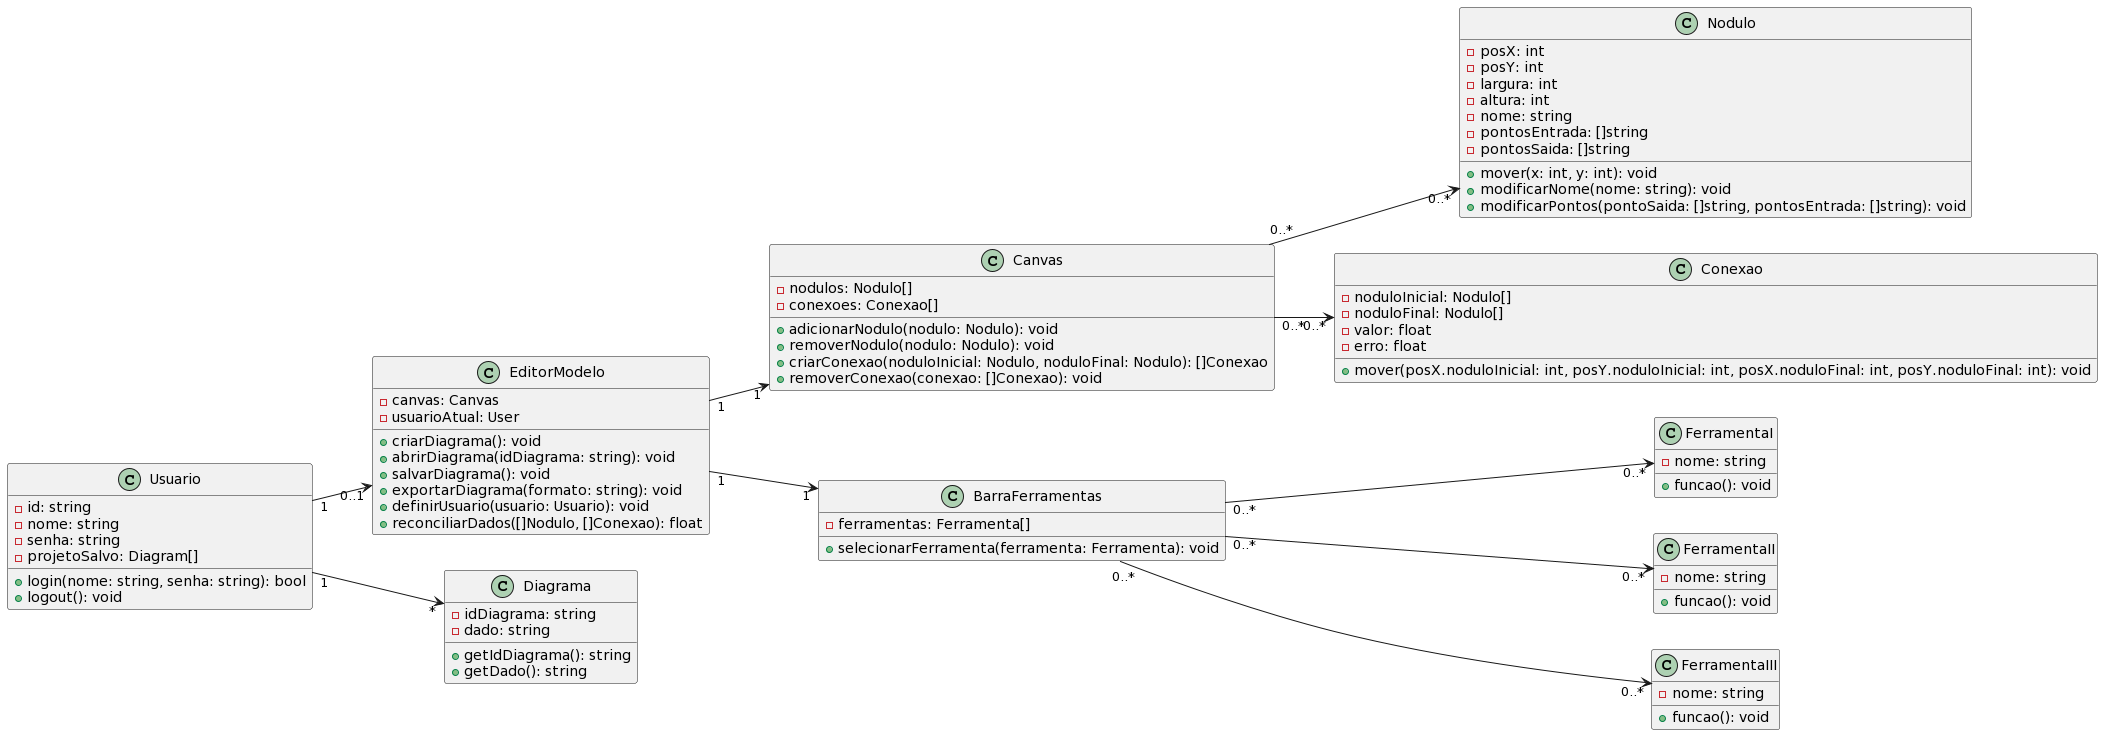
\includegraphics[width=0.6\textwidth]{figuras/ClassDiagram.png}
    \end{center}
\end{figure}
            
Adicionalmente, os relacionamentos entre as classes são destacados por meio de linhas que conectam os blocos das classes. Essas associações podem assumir diferentes formas, como associações simples, agregações, composições, heranças, entre outras, e fornecem \textit{insights} valiosos sobre como as diferentes partes do sistema interagem e dependem umas das outras.
            
Assim, um diagrama de classes torna-se uma ferramenta essencial para modelar a estrutura estática de um sistema, oferecendo uma representação visual nítida das classes, atributos, métodos e seus inter-relacionamentos, o que simplifica o processo de \textit{design}, análise e comunicação entre os integrantes da equipe de desenvolvimento de \textit{software} \cite{softwareenguml}.
            
% -------------------------
\subsubsection{Diagrama de caso de uso}
        
O diagrama de caso de uso é uma representação visual amplamente utilizada na engenharia de \textit{software} para descrever a interação entre um sistema e seus usuários. Ele destaca os diferentes casos de uso, que representam as diferentes maneiras pelas quais os usuários interagem com o sistema para atingir seus objetivos. Na sua forma mais básica, um diagrama de caso de uso consiste em atores, que são os usuários externos ao sistema, e de casos de uso, que são as diferentes funcionalidades ou serviços oferecidos pelo sistema, como exemplificado no diagrama da Figura \ref{fig:UseCaseDiagram}.
        
\begin{figure}[htb]
    \caption{\label{fig:UseCaseDiagram}Diagrama de Caso de Uso em UML.}
    \begin{center}
        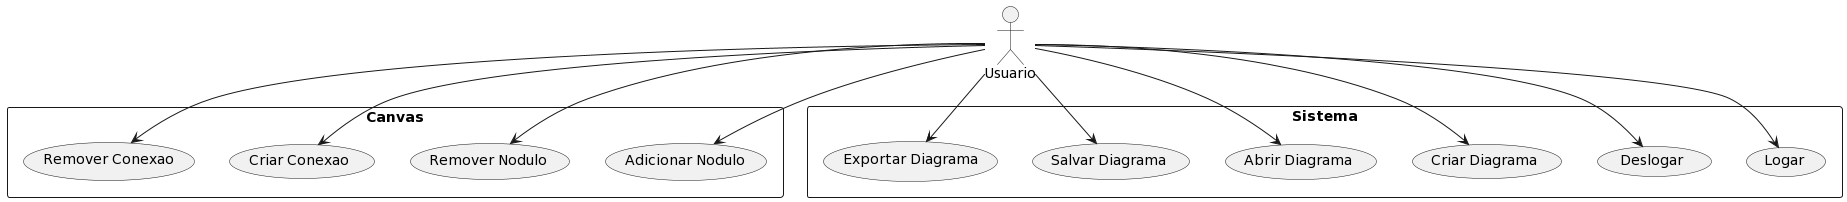
\includegraphics[width=0.6\textwidth]{figuras/UseCaseDiagram.png}
    \end{center}
\end{figure}
        
Os atores representam os diferentes tipos de usuários que interagem com o sistema, enquanto os casos de uso representam as diferentes funcionalidades oferecidas pelo sistema. Esses casos de uso são conectados aos atores por meio de linhas, indicando a interação entre os usuários e as funcionalidades do sistema.
        
Assim, um diagrama de caso de uso torna-se uma ferramenta essencial para modelar a interação entre um sistema e seus usuários, oferecendo uma representação visual clara dos atores, casos de uso e seus inter-relacionamentos. Isso simplifica o processo de \textit{design}, análise e comunicação entre os membros da equipe de desenvolvimento de \textit{software}, garantindo uma implementação eficaz e orientada às necessidades dos usuários.

% -------------------------
\subsubsection{Diagrama do banco de dados}

O diagrama de banco de dados é uma representação visual das estruturas de dados e dos relacionamentos entre elas em um sistema de banco de dados \cite{databasedepth}, na qual visa representar a estrutura dos dados armazenados em um banco de dados e como esses dados estão relacionados entre si, como é o caso da Figura \ref{fig:DatabaseDiagram}, que representa o banco de dados do sistema.
            
\begin{figure}[htb]
    \caption{\label{fig:DatabaseDiagram}Diagrama de Banco de Dados em UML.}
    \begin{center}
        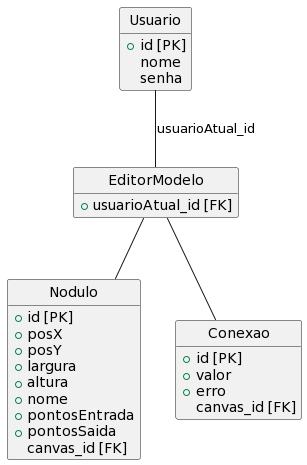
\includegraphics[width=0.6\textwidth]{figuras/DatabaseDiagram.png}
    \end{center}
\end{figure}
            
No diagrama de banco de dados, as entidades são representadas por tabelas, onde cada tabela possui colunas que representam os atributos dos dados armazenados. Além disso, as relações entre as tabelas são representadas por meio de chaves estrangeiras, indicando como os dados de uma tabela estão relacionados aos dados de outra tabela.
            
Desta forma, um diagrama de banco de dados é uma ferramenta vital para modelar a estrutura dos dados em um sistema de banco de dados, oferecendo uma representação visual clara das tabelas, colunas e relacionamentos entre elas. Isso facilita o projeto, análise e comunicação entre os membros da equipe de desenvolvimento de \textit{software}, garantindo uma implementação eficiente e eficaz do sistema de banco de dados.

% -------------------------
\section{Versionamento no desenvolvimento do software}

Para o desenvolvimento do RADARE, foram utilizados \textit{Git} e \textit{GitHub} como ferramentas de versionamento de código e controle de colaboração. O \textit{Git} é um sistema de controle de versão distribuído que permite rastrear e gerenciar alterações no código ao longo do tempo, possibilitando que os desenvolvedores trabalhem em diferentes partes do projeto de forma paralela sem conflitos. Essa ferramenta facilita o processo de desenvolvimento incremental, pois permite o registro de cada modificação e a reversão de alterações caso sejam detectados erros.

\textit{GitHub}, por sua vez, é uma plataforma baseada em nuvem que hospeda repositórios \textit{Git}, facilitando a colaboração e integração de código entre os membros da equipe. Além de oferecer um ambiente centralizado para o armazenamento seguro dos arquivos do projeto, \textit{GitHub} disponibiliza ferramentas que automatizam o processo de revisão de código, como \textit{pull requests} e \textit{code reviews}. Essas funcionalidades permitem que os membros da equipe possam revisar e discutir as mudanças antes de serem integradas ao código principal, garantindo a qualidade e a consistência do projeto.

Adicionalmente, o uso de \textit{branches} em \textit{Git} permite que cada nova funcionalidade ou correção seja desenvolvida isoladamente, sendo integrada ao código principal somente após validação. Esse fluxo de trabalho facilita o gerenciamento de versões e minimiza o risco de conflitos, além de permitir o rastreamento detalhado do progresso do desenvolvimento.

% -------------------------
\section{Ambiente de desenvolvimento do software}

O desenvolvimento do RADARE foi realizado em um ambiente configurado para otimizar a produtividade e a organização dos componentes do sistema. O editor de código \textit{Visual Studio Code (VSCode)} foi utilizado como ferramenta principal, devido à sua interface intuitiva e suporte a extensões, facilitando a escrita e organização do código. O sistema operacional utilizado foi o \textit{Windows 11}, que ofereceu um ambiente estável e compatível com as ferramentas empregadas no projeto.

Para testar e garantir a compatibilidade do \textit{website}, foram utilizados os navegadores \textit{Microsoft Edge}, \textit{Google Chrome} e \textit{Mozilla Firefox}. Essa abordagem permitiu avaliar o comportamento e a responsividade da interface em diferentes navegadores, assegurando que o sistema fosse acessível e funcional para uma variedade de usuários.

Informações detalhadas sobre a configuração da máquina utilizada no desenvolvimento do sistema, incluindo especificações de hardware e software, estão disponíveis no \textbf{Apêndice \ref{Ap:configuracaoMaquina}}. Esse ambiente de desenvolvimento foi fundamental para a construção e testes do RADARE, proporcionando as ferramentas necessárias para uma implementação eficiente e controle visual de qualidade.

    
% -------------------------
\section{Linguagem TypeScript no desenvolvimento do front-end}

No desenvolvimento do front-end do RADARE, o TypeScript foi escolhido como a linguagem principal devido à sua tipagem estática opcional, que adiciona estrutura e robustez ao código em comparação ao JavaScript. Com o TypeScript, foi possível definir tipos específicos para variáveis, funções e objetos, reduzindo a ocorrência de erros de tipo e facilitando a detecção de problemas ainda na fase de desenvolvimento. Além disso, o uso de interfaces e classes trouxe uma organização clara dos componentes, promovendo a reutilização de código e facilitando a implementação modular.

A estrutura do projeto foi baseada em uma abordagem modular, onde cada componente foi desenvolvido como uma unidade independente. Isso facilitou a manutenção e a escalabilidade, especialmente para os elementos visuais do \textit{canvas}, onde cada nódulo e conexão pode ser manipulado de forma individual. A tipagem garantiu que todos os elementos do \textit{canvas} tivessem propriedades definidas, como posição e estado, assegurando interações consistentes entre os módulos.

Para a construção da interface visual, o TypeScript foi integrado ao HTML e SCSS, com o HTML definindo a estrutura dos elementos e o SCSS cuidando do design e layout. O TypeScript coordenou as interações entre a interface e a lógica de negócios, tornando a interface responsiva e interativa, reagindo às entradas do usuário de maneira dinâmica.

% -------------------------
\section{Linguagem Python no desenvolvimento do \textit{back-end}}

A linguagem \textit{Python} foi escolhida para o desenvolvimento do \textit{back-end} do RADARE devido à sua simplicidade, flexibilidade e à ampla variedade de bibliotecas disponíveis, que facilitam a implementação de funcionalidades essenciais em sistemas de reconciliação de dados. Python é reconhecido pela sua clareza e legibilidade, características que tornam o desenvolvimento mais eficiente e reduzem o tempo necessário para depuração e manutenção do código. Além disso, o suporte robusto a cálculos numéricos e estatísticos através de bibliotecas como \textit{NumPy} e \textit{SciPy} permite realizar operações complexas de maneira otimizada, um aspecto crucial para o processamento de dados em tempo real.

Para a criação de uma API RESTful que facilita a comunicação entre o \textit{front-end} e o banco de dados, foi utilizado o microframework \textit{Flask}. \textit{Flask} é uma ferramenta leve e modular que oferece flexibilidade para a construção de aplicações \textit{web} sem impor uma estrutura rígida. Essa flexibilidade é vantajosa no desenvolvimento do RADARE, pois permite a implementação de \textit{endpoints} customizados para manipulação de dados, que se ajustam facilmente às necessidades específicas do sistema de reconciliação.

Além disso, \textit{Flask} integra-se perfeitamente com \textit{Psycopg2}, uma biblioteca que permite conectar o \textit{Python} ao banco de dados \textit{PostgreSQL}. Essa integração possibilita que os dados sejam armazenados e recuperados com segurança e eficiência, mantendo a integridade dos dados durante todo o processo de manipulação. A simplicidade do \textit{Flask}, combinada com a robustez do \textit{Python}, oferece um ambiente ágil para o desenvolvimento de aplicações orientadas a dados, onde a confiabilidade e o desempenho são essenciais.

Essas qualidades, somadas à vasta comunidade de desenvolvedores que continuamente aprimoram e documentam recursos em \textit{Python} e \textit{Flask}, fazem dessa combinação uma escolha ideal para o desenvolvimento do \textit{back-end} de sistemas como o RADARE. O resultado é uma aplicação ágil, escalável e capaz de gerenciar grandes volumes de dados com alta precisão.
    
% -------------------------
\section{Ferramenta PostgreSQL no desenvolvimento do banco de dados}

Para o desenvolvimento do banco de dados do RADARE, foi escolhido o \textit{PostgreSQL} devido à sua robustez, confiabilidade e capacidade de lidar com grandes volumes de dados de forma eficiente. O \textit{PostgreSQL} é um sistema de gerenciamento de banco de dados relacional de código aberto, amplamente reconhecido por seu suporte a transações complexas e integridade de dados. Além disso, ele oferece uma variedade de tipos de dados e a capacidade de realizar operações avançadas, o que é fundamental para um sistema de reconciliação de dados.

Uma das principais vantagens do \textit{PostgreSQL} é o seu suporte a transações ACID (Atomicidade, Consistência, Isolamento e Durabilidade), garantindo que todas as operações realizadas no banco de dados sejam executadas de forma segura e consistente. Esse recurso é especialmente importante no contexto do RADARE, onde a precisão e integridade dos dados são essenciais para que os cálculos de reconciliação sejam confiáveis.

Além disso, o \textit{PostgreSQL} permite a criação de \textit{views} e \textit{stored procedures}, facilitando a organização dos dados e melhorando o desempenho das consultas. Essa capacidade de definição de lógica no banco de dados possibilita uma interação mais eficiente entre o \textit{back-end} e o banco, uma vez que parte do processamento pode ser realizada diretamente no nível do banco de dados, reduzindo a carga de processamento no servidor.

O suporte a integrações com bibliotecas como \textit{Psycopg2} também permite que o \textit{PostgreSQL} seja facilmente conectado ao \textit{back-end} em \textit{Python}, garantindo uma comunicação rápida e segura entre o sistema e o banco de dados. Essa compatibilidade torna o \textit{PostgreSQL} uma escolha ideal para o RADARE, permitindo o armazenamento e recuperação de dados de forma escalável, eficiente e segura.
   
